\chapter{基于web可视化工具概述}
\chaptermark{基于web可视化工具概述}
	\section{GBrowse}
		\subsection{概述}
		GBrowse是基因组浏览器(GenomeBrowse)的缩写。它是一种基于WE
		\subsection{可视化方式}
		GBrowse用 track的方式进行可视化相关基因组信息,通过对track进行缩放。通过合理地配置及编码可以实现基因组基因的可视化。
	
		\subsection{可视化内容}
		GBrowse可视化内容由可视化图谱进行具体显示,可视化图谱可以分为三个部分:overview(概述),region(区域),details(细节)。
		\begin{itemize}
			\item 计算机用户必须要树立正确的病毒防范观念,应该对目前互联网上的病毒传播手段有一定的了解,对病毒防范知识要有一定的掌握。
			\item 计算机用户必须要树立正确的病毒防范观念,应该对目前互联网上的病毒传播手段有一定的了解,对病毒防范知识要有一定的掌握。
			\item 计算机用户必须要树立正确的病毒防范观念,应该对目前互联网上的病毒传播手段有一定的了解,对病毒防范知识要有一定的掌握。
		\end{itemize}

		\begin{figure}
			\centering
			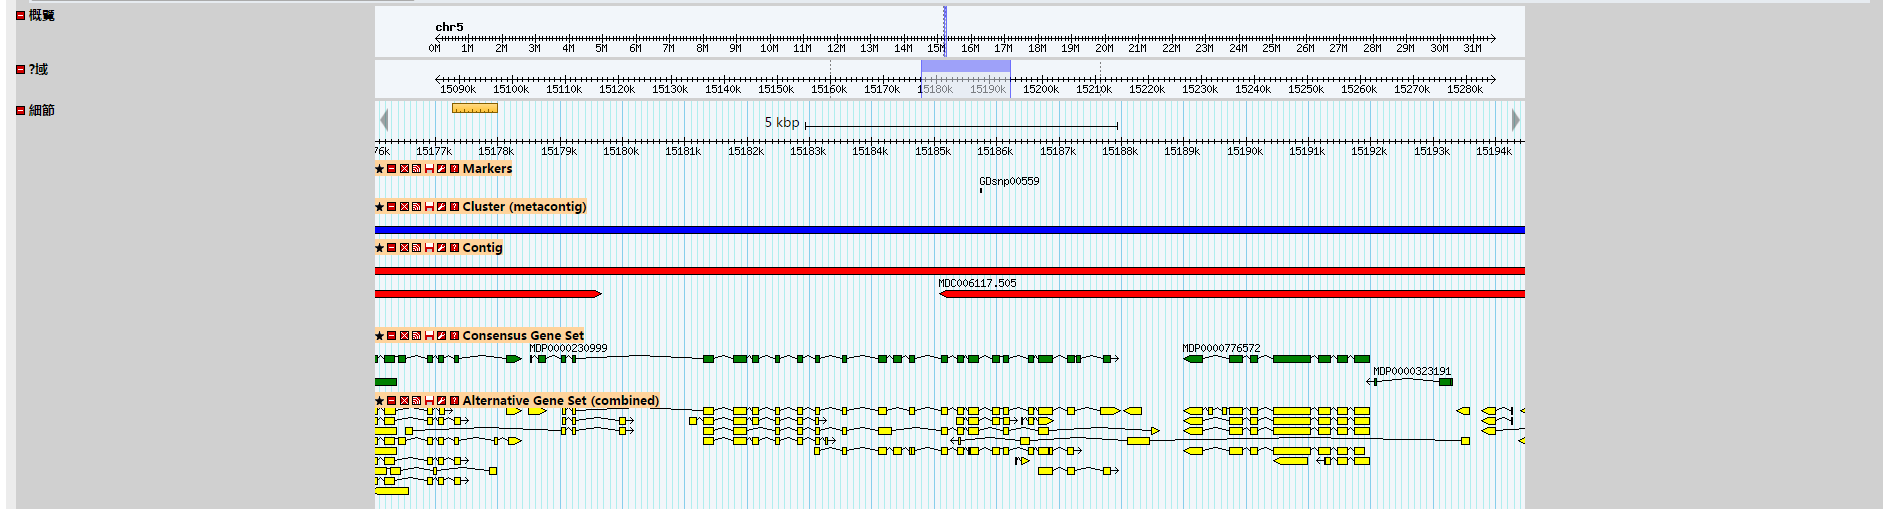
\includegraphics[width = .9\textwidth]{2-1.png}
			\caption{GBrowse页面内容展示图}
		\end{figure}	
		\subsection{系统架构}
			计算机用户必须要树立正确的病毒防范观念,应该对目前互联网上的病毒传播手段有一定的了解,对病毒防范知识要有一定的掌握。互联网中有很多充满诱惑的内容,对于这些极有可能存在病毒的内容,用户必须要增强自己的控制能力,在互联网上下载的各种资料数据在打开和使用之前应该用杀毒软件进行扫描,同时养成良好的计算机操作习惯,这样一来病毒自然就会远离我们。另外,我们还可以通过截断病毒的传播途径来防范病毒。计算机病毒具有极强的传播性,在计算机网络中,如果没有采取有效的防范措施来阻挡其传播途径,那么病毒就会在很短的时间内对局域网、服务器、互联网造成危害。如果处于一个局域网中的某一台计算机受到感染,那么应该立刻断网,对其进行隔离,终止对于这台计算机共享文件的使用,这样一来就能够很好的切断病毒的传播途径,防止病毒危害其他计算机。
		\begin{figure}[!ht]
			\centering
			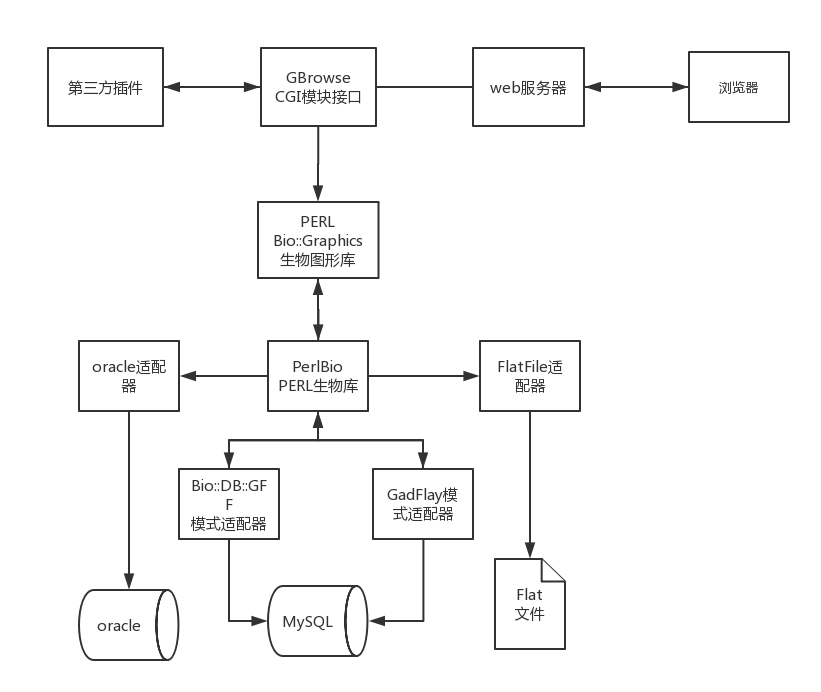
\includegraphics[width = .6\textwidth]{2-2.png}
			\caption{GBrowse系统结构}
		\end{figure}
		\subsection{运行机理}
			计算机用户必须要树立正确的病毒防范观念,应该对目前互联网上的病毒传播手段有一定的了解,对病毒防范知识要有一定的掌握。互联网中有很多充满诱惑的内容,对于这些极有可能存在病毒的内容,用户必须要增强自己的控制能力,在互联网上下载的各种资料数据在打开和使用之前应该用杀毒软件进行扫描,同时养成良好的计算机操作习惯,这样一来病毒自然就会远离我们。另外,我们还可以通过截断病毒的传播途径来防范病毒。计算机病毒具有极强的传播性,在计算机网络中,如果没有采取有效的防范措施来阻挡其传播途径,那么病毒就会在很短的时间内对局域网、服务器、互联网造成危害。如果处于一个局域网中的某一台计算机受到感染,那么应该立刻断网,对其进行隔离,终止对于这台计算机共享文件的使用,这样一来就能够很好的切断病毒的传播途径,防止病毒危害其他计算机。
			\begin{figure}[!ht]
				\centering
				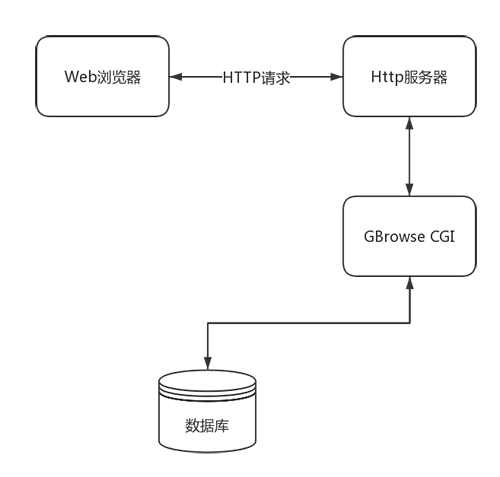
\includegraphics[width = .5\textwidth]{2-3.png}
				\caption{GBrowse模块请求处理}
			\end{figure}
		\subsection{优缺点}
			计算机用户必须要树立正确的病毒防范观念,应该对目前互联网上的病毒传播手段有一定的了解,对病毒防范知识要有一定的掌握。互联网中有很多充满诱惑的内容,对于这些极有可能存在病毒的内容,用户必须要增强自己的控制能力,在互联网上下载的各种资料数据在打开和使用之前应该用杀毒软件进行扫描,同时养成良好的计算机操作习惯,这样一来病毒自然就会远离我们。另外,我们还可以通过截断病毒的传播途径来防范病毒。计算机病毒具有极强的传播性,在计算机网络中,如果没有采取有效的防范措施来阻挡其传播途径,那么病毒就会在很短的时间内对局域网、服务器、互联网造成危害。如果处于一个局域网中的某一台计算机受到感染,那么应该立刻断网,对其进行隔离,终止对于这台计算机共享文件的使用,这样一来就能够很好的切断病毒的传播途径,防止病毒危害其他计算机。
		%JBrowse
	\section{JBrowse}
		\subsection{概述}
			台应用开发框架下逐步推出Windows等操作系统下的应用软件,方便用户可视化数据。
		\subsection{可视化方式}
			JBrowse用 track 的方式进行可视化,提供平滑的动态移动和缩放功能,也有导航和通道的选择。JBrowse可以展示多种 track 视图,除基本视图外,还可以显示非翻译区、外显子、内含子结构等。
		
		\subsection{可视化内容}
			JBrowse可以展示基因组整体视图,也可以细化展示基因跨度、tRNA、转座子、寡核苷酸、蛋白质结合位点、增强子、基因调控区域、非编码RNA、点突变、序列变异信息等其它基因信息。用户可以自己上传需要可视化的内容的相关基因数据,支持GFF、GFF3、WIG、BED、FASTA、Wiggle、BigWig、BAM 等多种格式的数据文件。如图2-5所示
		\begin{figure}[!ht]
			\centering
			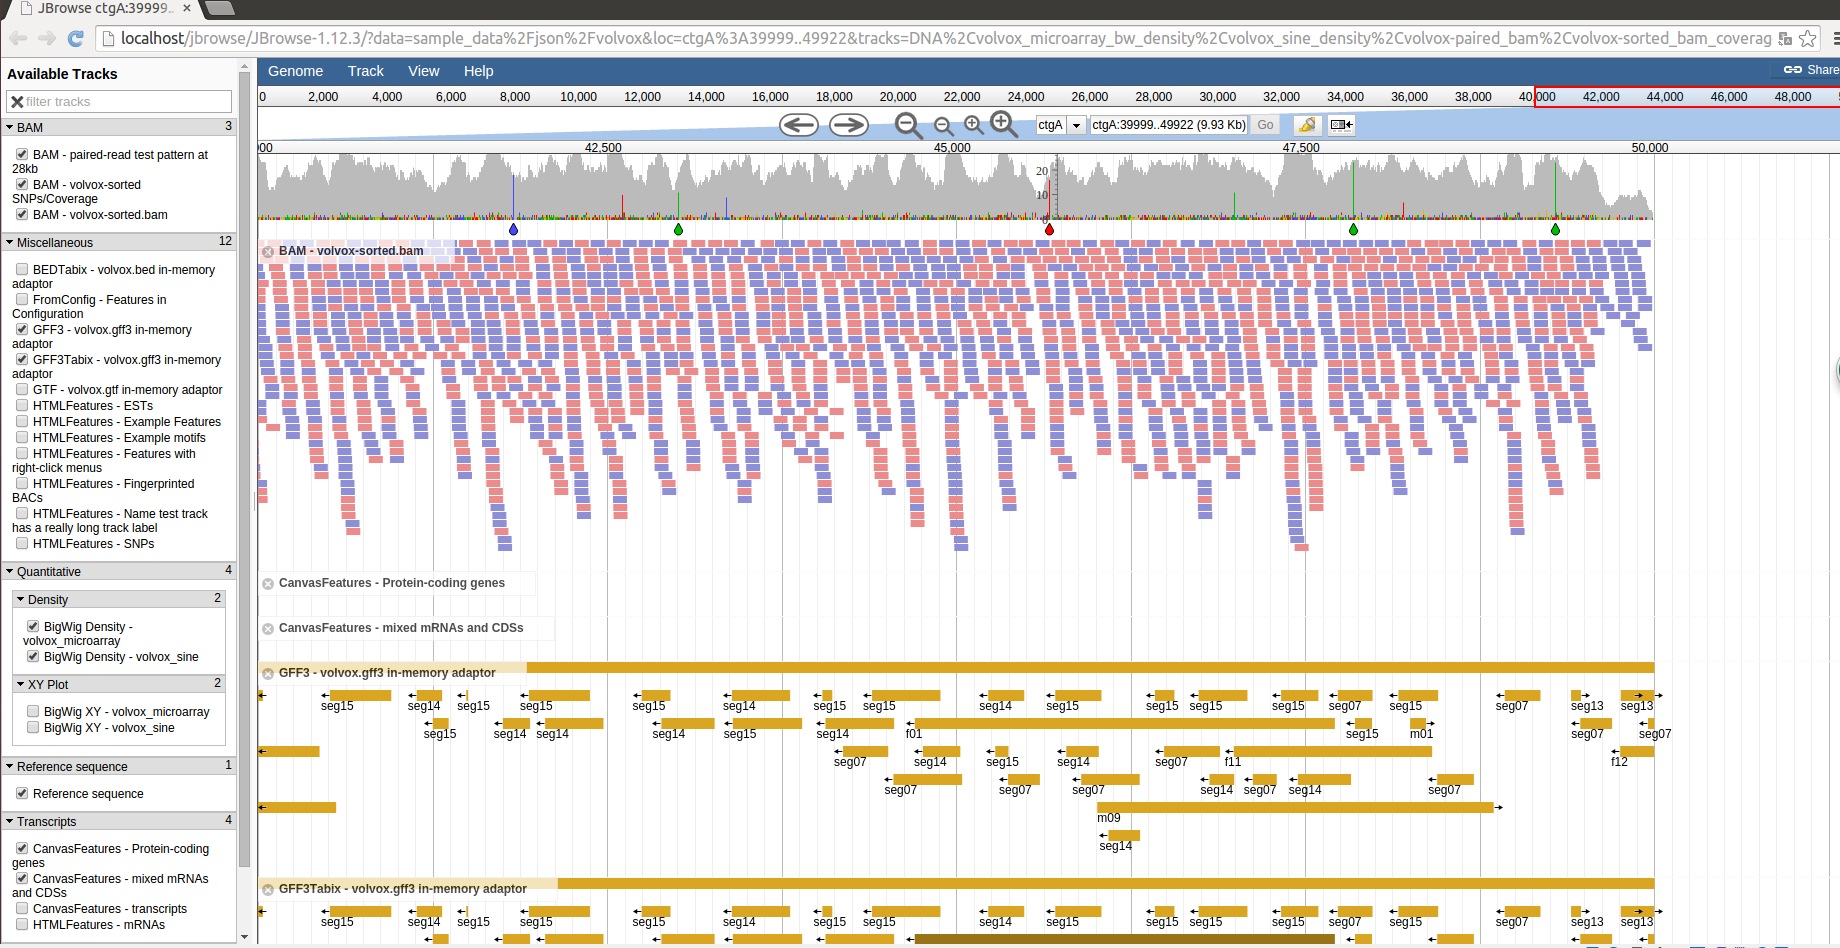
\includegraphics[width = .6\textwidth]{2-4.png}
			\caption{JBrowse可视化内容}
		\end{figure}
		\subsection{系统架构}
			对于计算机病毒的防范,单单依靠技术手段是不能彻底解决问题的,因此必须要把技术和管理结合在一起,这是现阶段病毒防范的主流方法。因为计算机病毒的防范措施,从目前的实际情况来看依旧是非常被动的,人工智能的结合病毒防范技术依旧仅仅停留在实验室阶段,并没有推广和普及。而就网络管理来说,我们可以主动的出击,按照计算机病毒的感染机制,对计算机进行正确的操作和使用,制定完善的网络访问规范,对于服务器进行定期的杀毒和维护,最大限度的预防病毒的侵害。通过对计算机使用的规范化,可以在很大程度上避免用户对不良网站、信息的点击,可以有效的避免一些利用诱惑性图片来吸引用户点击的非法网站,从而预防病毒对计算机的入侵。
		\begin{figure}[!ht]
			\centering
			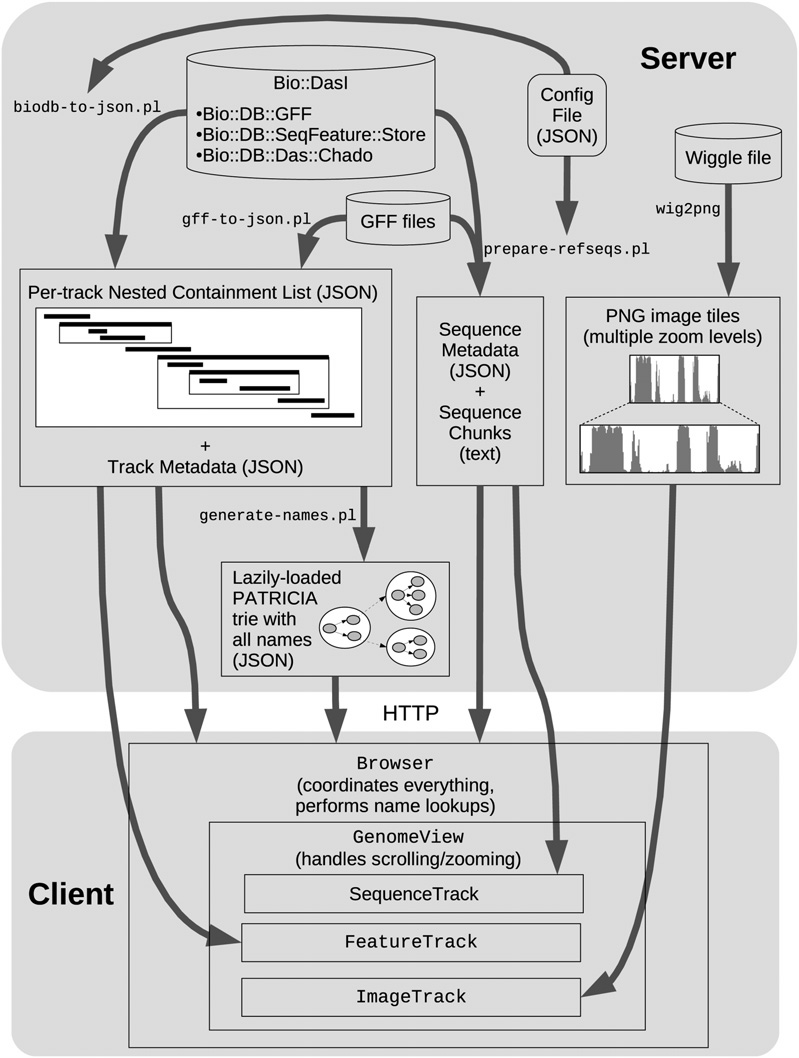
\includegraphics[width = .4\textwidth]{2-5.png}
			\caption{JBrowse系统架构}
		\end{figure}
		\subsection{运行机理}
		第一,导致计算机运行缓慢。当病毒程序执行的过程中,不但会占据计算机内存,还会干扰系统的正常运行,导致系统运行缓慢。虽然说这样的危害从表面上来看并不会给系统带来较大的损失,但是在用户使用计算机的过程中,会不断的消耗计算机系统的资源,最终甚至可能导致系统的停止运行。

		第二,病毒会大量占用系统内存以及计算机磁盘空间。当计算机感染某些病毒之后,硬盘会自动开始持续性的读取,虽然用户并未执行操作,但是硬盘却处于高速运转状态,计算机内存也被大量的占用。此外,某些文件型病毒甚至可能在短时间内感染大量的系统文件,从而让用户硬盘中产生大量的垃圾文件,极大的占据了硬盘空间。

		第三,对计算机数据进行破坏。病毒极有可能篡改计算机系统设置或者对计算机系统进行加密的方法,从而引起计算机系统的混乱,更严重的时候会破坏计算机的硬盘引导区,造成计算机无法正常启动等。第四,病毒所带来的垃圾信息会对用户计算机网络造成一定的危害,甚至可能导致网络瘫痪现象。例如当计算机感染蠕虫病毒之后,在用户不知情的情况下,病毒会让计算机向外发送大量垃圾邮件或数据,从而让网络严重堵塞或瘫痪。最近几年以来,很多不法分子通过即时通讯软件向用户发送大量带有病毒的垃圾信息和邮件,成为了病毒传播的一种新的途径。

		第五,窃取用户的各种隐私。当前,很多计算机用户对于木马病毒已经是深恶痛绝。有关调查显示,当前木马病毒占据了计算机病毒的60\%左右,其中大部分木马病毒的传播目的都是为了窃取用户的个人信息从而帮助病毒制造者获取非法利益。用户信息一旦泄露,将会给用户带来不可估量的损失。
		\begin{figure}[!ht]
			\centering
			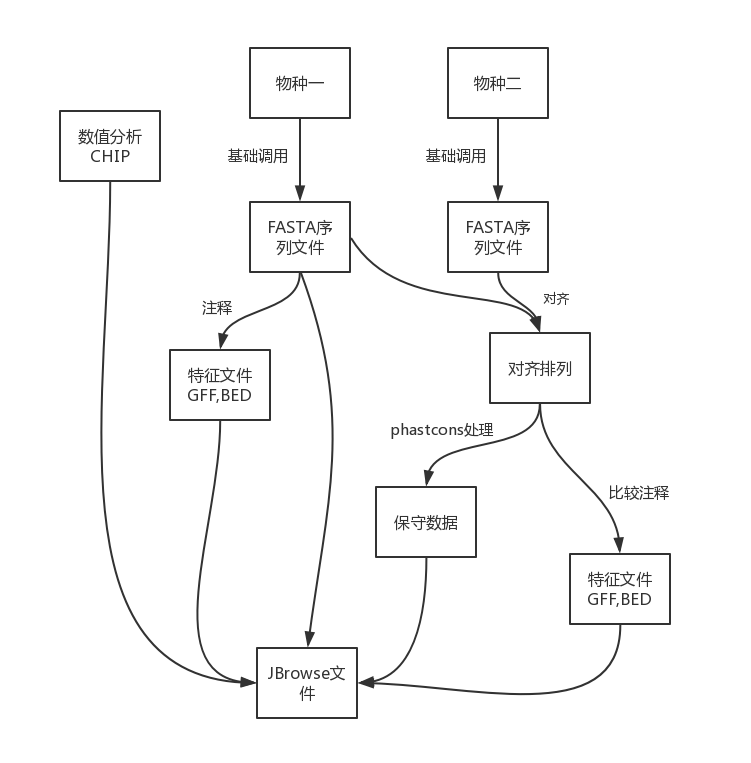
\includegraphics[width = .4\textwidth]{2-6.png}
			\caption{JBrowse工作流图}
		\end{figure}
		\subsection{优缺点}
		优点:流浏览器对 HTML5 中新标签的支持不完善,造成用户体验不佳等问题。
	\section{UCSC Genome Browser}		
			\subsection{概述}	
			 按照病毒的存在媒体进行分类,一般可以分为引导型、文件型和混合型三种类型。引导型病毒一般来说主要藏匿于磁盘引导区,当电脑启动之后,隐藏在磁盘的病毒便会开始传播;文件型的病毒常常会对计算机中的可执行文件进行感染,例如com、exe、doc文件;而混合型病毒属于上述两种病毒的混合型,其算法复杂,传播的途径和危害更大。
			\subsection{可视化方式}		
			 按照病毒的存在媒体进行分类,一般可以分为引导型、文件型和混合型三种类型。引导型病毒一般来说主要藏匿于磁盘引导区,当电脑启动之后,隐藏在磁盘的病毒便会开始传播;文件型的病毒常常会对计算机中的可执行文件进行感染,例如com、exe、doc文件;而混合型病毒属于上述两种病毒的混合型,其算法复杂,传播的途径和危害更大。
			\begin{figure}[!ht]
				\centering
				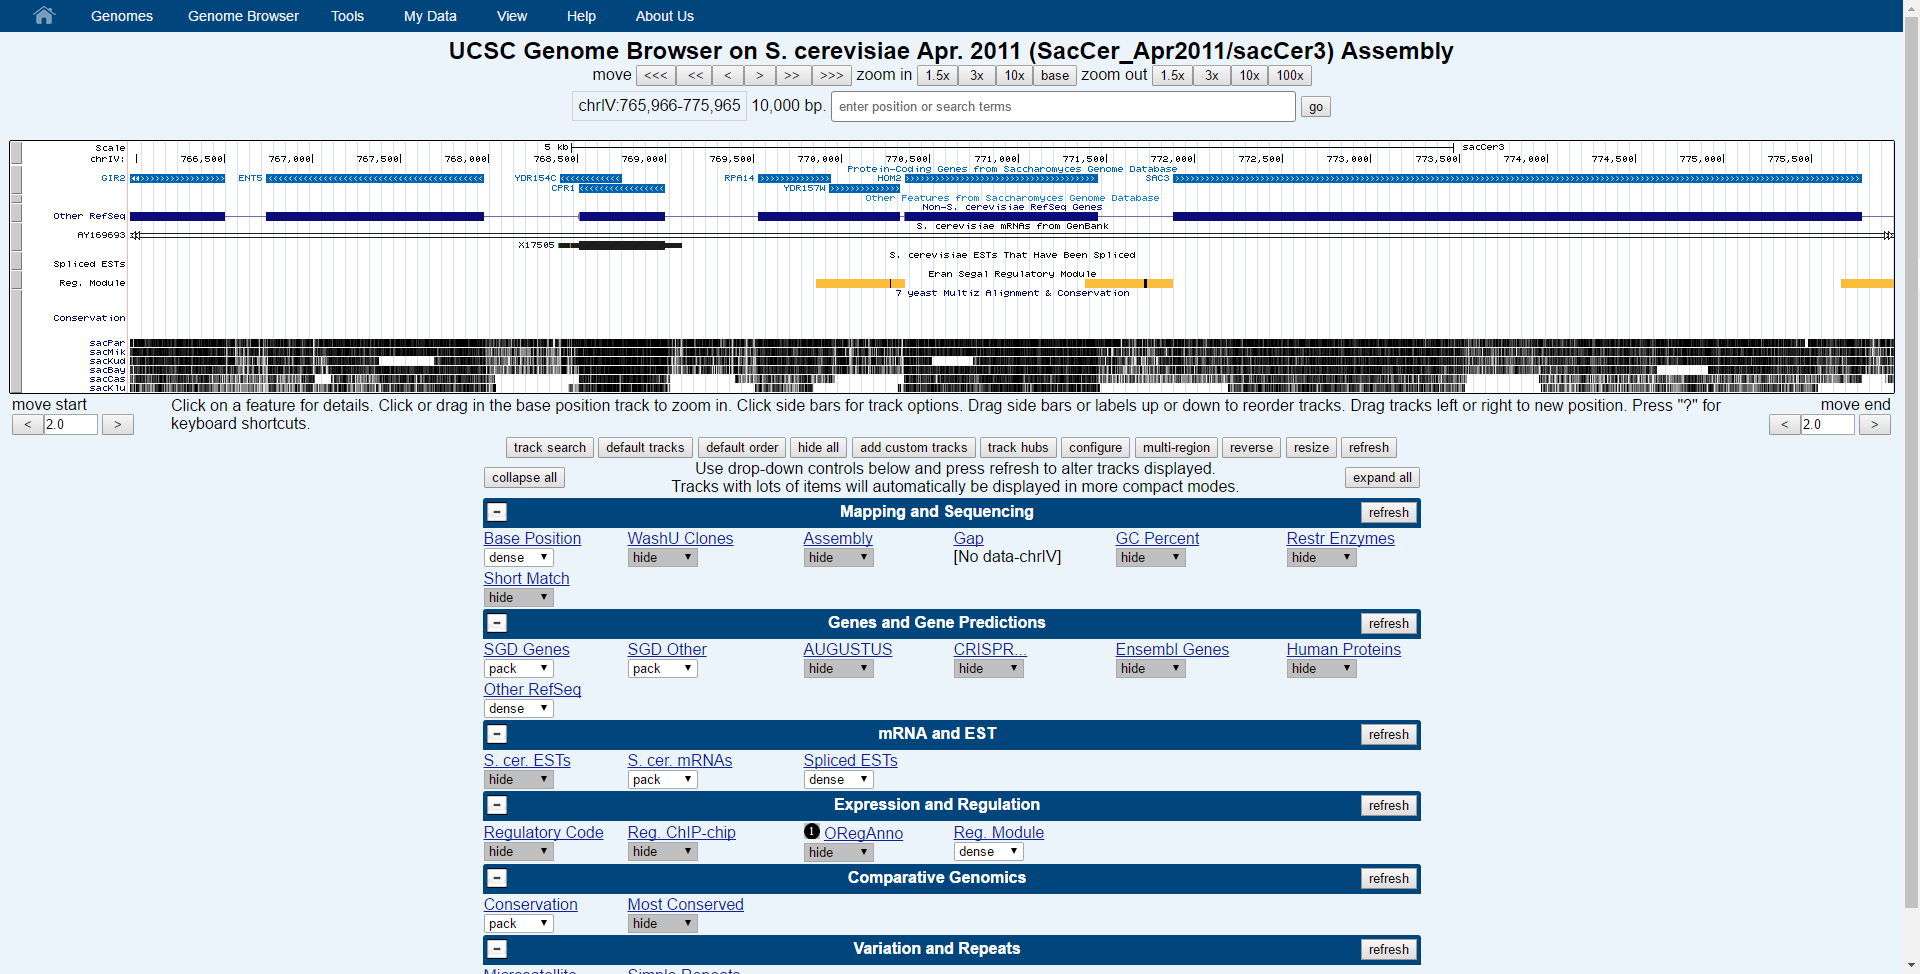
\includegraphics[width = .4\textwidth]{2-7.png}
				\caption{UCSC Genome Browser系统界面}
			\end{figure}
			\subsection{可视化内容}		
			 按照病毒的存在媒体进行分类,一般可以分为引导型、文件型和混合型三种类型。引导型病毒一般来说主要藏匿于磁盘引导区,当电脑启动之后,隐藏在磁盘的病毒便会开始传播;文件型的病毒常常会对计算机中的可执行文件进行感染,例如com、exe、doc文件;而混合型病毒属于上述两种病毒的混合型,其算法复杂,传播的途径和危害更大。
			\subsection{系统架构}		
			工作站是直接面向互联网的,大多数的病毒都是首先通过工作站传播到整个网络中去的。现阶段工作站对病毒的防范措施主要有三种:第一是软件防范,这种防范方法相对简单,它通过在工作站上安装最新的杀毒软件就能够起到预防病毒入侵的目的。需要注意的是,使用这种方法必须要及时的对杀毒软件的病毒库进行升级,这样才能够预防更多的已知病毒;第二是在工作站上插入病毒卡,选择这种病毒防范措施的有点是可以实现对病毒入侵的实时监测,进一步的增强工作站病毒防范能力。但是这种方式的缺点也比较突出,它会占据一部分系统资源,从而导致系统运行速度变慢,而且病毒卡的升级更新相对来说也比较困难;第三是在网络接口上装病毒防御芯片,它可以把工作站与服务器的存储控制和病毒防御结合在一起,进一步增强计算机病毒的实时防御。另外这种防范措施也在一定程度上增强了服务器的安全性,但是这种方法也存在一个升级更新不便的问题。因此当前选择最多的防范措施依旧是安装杀毒软件。
			\subsection{优缺点}
			计算机病毒属于人为编写的,直接感染计算机系统同时对系统资产造成危害的一种程序,从本质上来说计算机病毒属于一个拥有自我复制能力的程序,它会对计算机软硬件造成较大的危害。病毒的种类非常多,而不同类型的病毒其危害程度和感染方式也不尽相同。一般来说我们主要将计算机病毒分为以下几种类型: